\header{2}
\chapter{Bootonderdelen \& Zeiltermen}
\section{Inleiding}
In dit hoofdstuk komen de verschillende onderdelen van de boot en een aantal zeiltermen aan bod. Deze termen en onderdelen zijn belangrijk om de volgende hoofdstukken in dit boek goed te begrijpen.

\section{Zeiltermen}
Voor duidelijke communicatie tijdens de les en in de boot is het van belang dat je een aantal zeiltermen kent. De belangrijkste termen worden hieronder besproken.

\subsection{Bakboord, Stuurboord, Loef en Lij}
Bakboord en stuurboord zijn het links en rechts \textbf{van de boot}, gezien vanaf het achterdek. Je moet altijd met de vaarrichting mee kijken. 

Loef en lij zeggen iets over de wind ten opzichte van je boot. De kant waar de wind de boot in komt, is de loefzijde, ook wel de hoge kant genoemd. De kant waar de wind de boot verlaat heet de lijzijde of lage kant. 
\begin{figure}[ht]
	\centering
	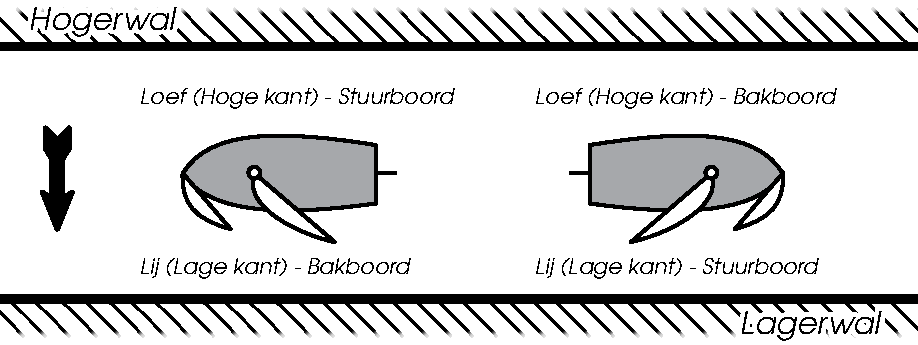
\includegraphics[width=0.9\textwidth]{Hoofdstukken/Onderdelen/pdf/wallen.pdf}
	\caption{Hoger- en Lagerwal}
	\centering
	\label{pic:hoog_laag}
\end{figure}

De hogerwal is de wal waar de wind vandaan komt. De lagerwal is de wal waar de wind naar toe waait. Al deze termen zijn te zien in figuur \ref{pic:hoog_laag}

\vfil\newpage

\subsection{Koersen}
Een koers vertelt iets over hoe je boot ligt ten opzichte van de wind. Alle koersen kun je zowel over bakboord, als stuurboord varen, behalve in de wind. Een overzicht van de koersen is te zien in figuur \ref{pic:koersen}. Wanneer je van koers verandert en naar de wind toe draait, loef je op. Wanneer je van de wind wegdraait heet dit afvallen. 

\begin{figure}[h]
	\centering
	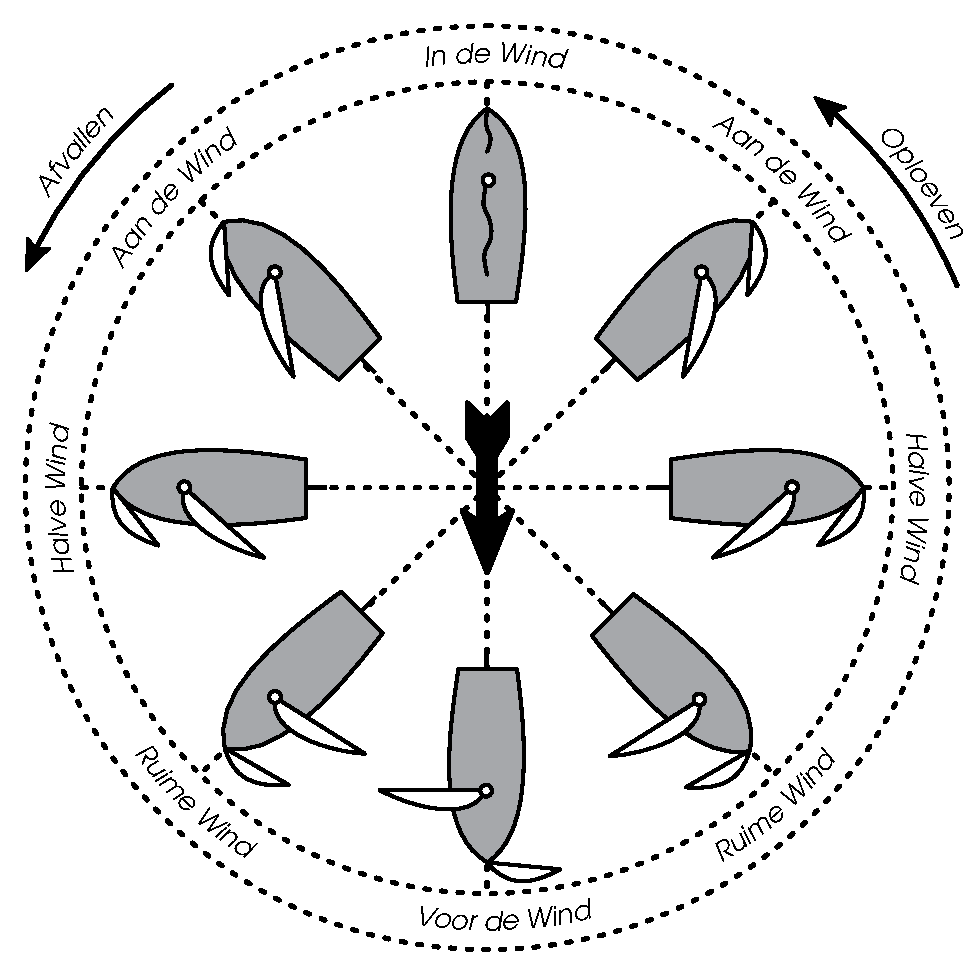
\includegraphics[width=0.9\textwidth]{Hoofdstukken/Onderdelen/pdf/koersen.pdf}
	\caption{Windkoersen}
	\label{pic:koersen}
\end{figure}



\subsection{Boven- en benedenwinds}
Op het water kan je vaak op twee manieren ergens langs varen: bovenwinds en benedenwinds. Bovenwinds houdt in dat je ergens langs vaart aan de kant waar de wind ernaartoe blaast, de hoge kant van het object. Benedenwinds is het tegenovergestelde: dit is de kant waar de wind van het object weg blaast en dus de lage kant van het object. Deze termen zijn te zien in figuur \ref{pic:boven_benedenwinds}.
\begin{figure}[h]
  \centering
  \begin{minipage}[b]{0.7\textwidth}
   \centering
    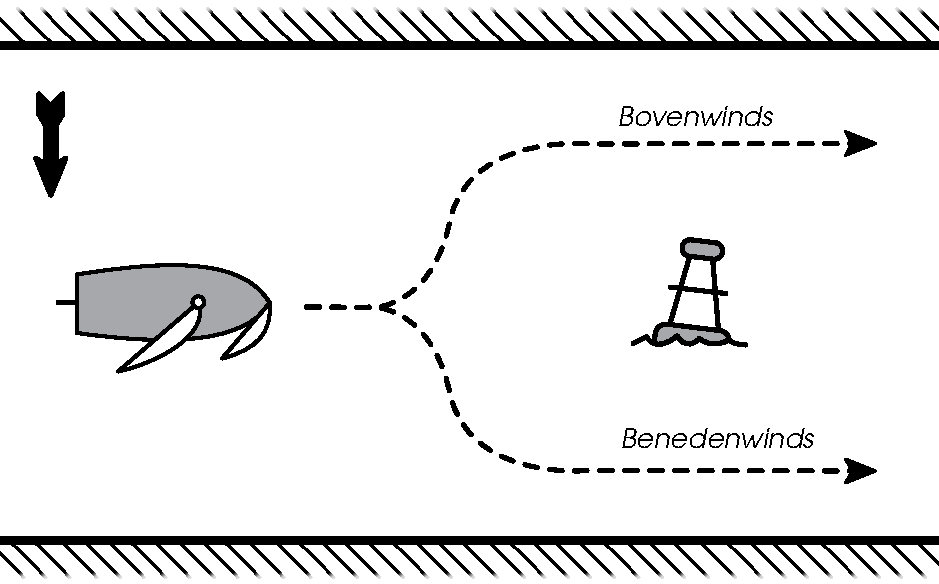
\includegraphics[width=0.9\textwidth]{Hoofdstukken/Onderdelen/pdf/boven_en_benedenwinds.pdf}
    \caption{Boven- en benedenwinds passeren van een boei}
    \centering
    \label{pic:boven_benedenwinds}
  \end{minipage}
  \hfill
  \begin{minipage}[b]{0.29\textwidth}
    \centering
    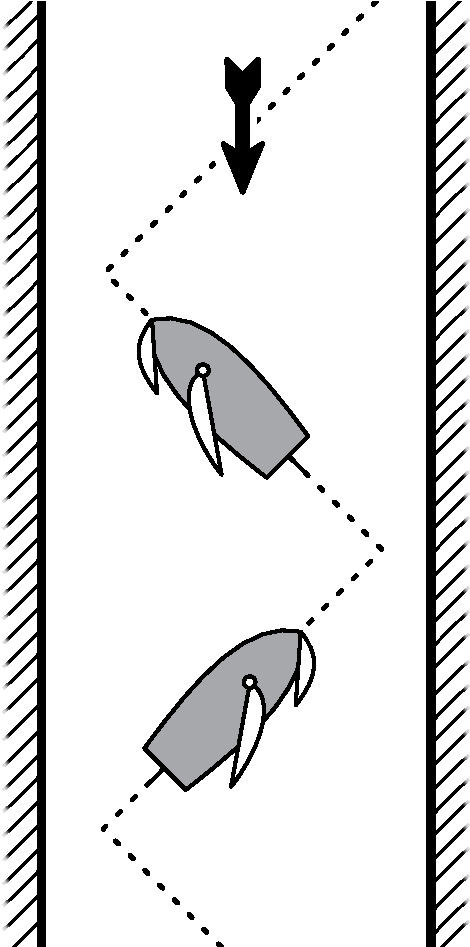
\includegraphics[width=0.7\textwidth]{Hoofdstukken/Onderdelen/pdf/opkruisen.pdf}
    \caption{Opkruisen}
    \label{pic:opkruisen}
  \end{minipage}
\end{figure}



Tip: De termen boven- en benedenwinds kunnen goed van pas komen bij een zeilwedstrijd. Hier wordt vaak aangegeven of je een boei boven- of benedenwinds moet ronden.

\newpage
\subsection{Overig}
Hiernaast dien je ook bekend te zijn met de onderstaande termen:

\begin{itemize}
    \item \textit{Overstag}: Je gaat hier van aan de wind over de ene boeg naar aan de wind over de andere boeg. Bijvoorbeeld: van aan de wind over bakboord naar aan de wind over stuurboord.
    \item \textit{Gijpen}: Je gaat hier van voor de wind over de ene boeg naar voor de wind over de andere boeg. Bijvoorbeeld: van voor de wind over bakboord naar voor de wind over stuurboord.
    \item \textit{Opkruisen of laveren}: Hierbij vaar je tegen de wind in door steeds aan de wind te varen en dan overstag te gaan. Een voorbeeld hiervan is te zien in figuur \ref{pic:opkruisen}
    \item \textit{Killen van het zeil}: Je laat dan expres een deel van je zeil minder wind vangen. Dit doe je door je zeil te vieren totdat alleen het achterlijk nog wind vangt.
    \item \textit{Opschieten}: Wanneer je een lijn opschiet, rol je deze netjes op. Ook wel bekend als opbossen.
    \item \textit{Beleggen}: Als je een kikker belegt, leg je de lijn via een bepaalde knoop op de kikker. Deze knoop zal in het hoofdstuk `Schiemannen' behandeld worden.
    \item \textit{Bak}: Wanneer je je fok bak doet, zet je deze aan de hoge kant in plaats van de lage kant.
    \item \textit{Deinzen}: Dit is wanneer je achteruit dobbert met de neus van je boot in de wind. 
\end{itemize}


\newpage

\section{Bootonderdelen}
In figuur \ref{pic:vlet_nummers} is een tekening van een lelievlet te zien met maar liefst 88 gelabelde onderdelen. De namen van de onderdelen staan in tabel \ref{table:vletwel}. Alle onderdelen, behalve die met grijze nummers, moet je kennen.

\begin{figure}[h!]
	\centering
	\makebox[\textwidth][c]{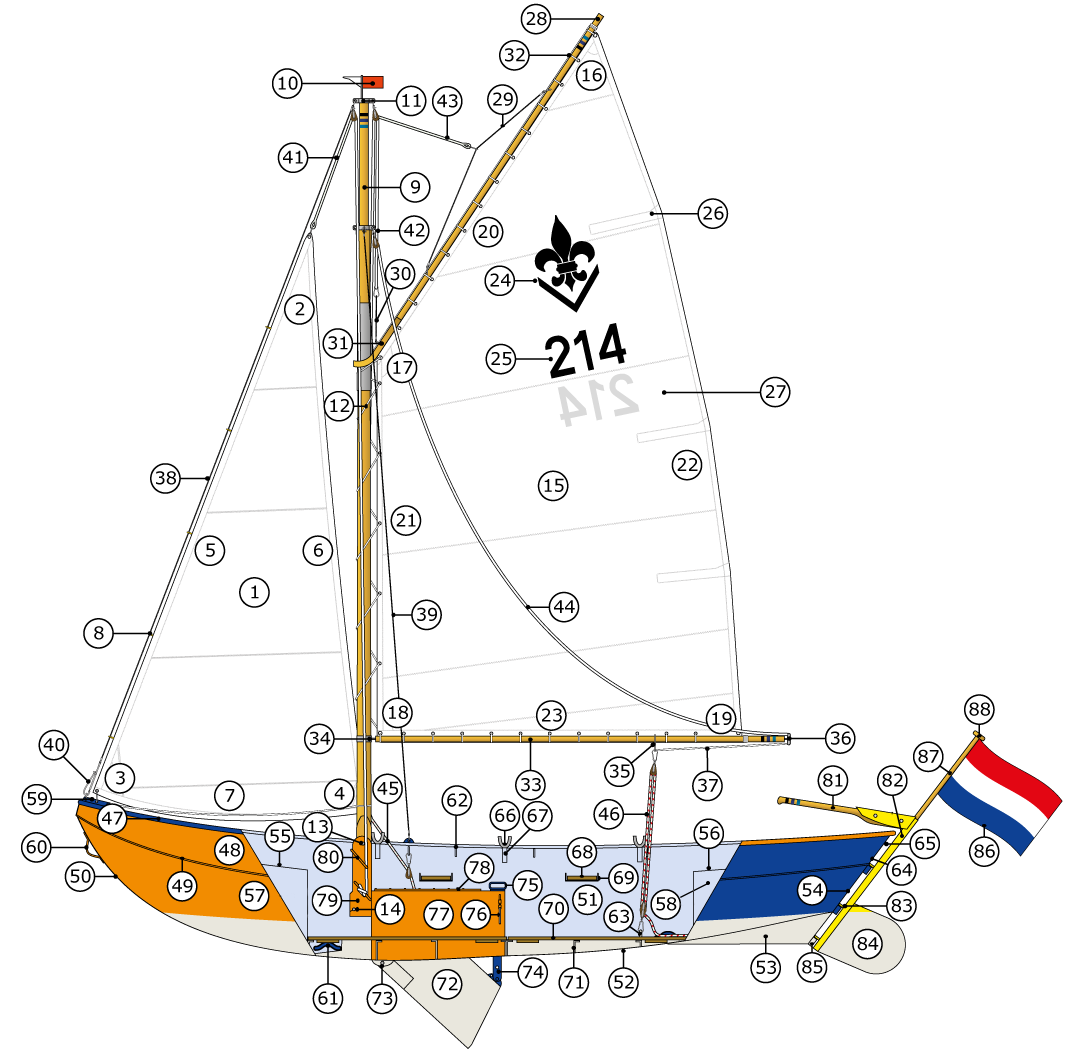
\includegraphics[width=1.2\textwidth]{Hoofdstukken/Onderdelen/png/lelievlet_onderdelen.png}}
	\caption{Tekening lelievlet met nummers \protect\footnotemark}
	\centering
	\label{pic:vlet_nummers}
\end{figure}

\footnotetext{\textit{Lelievlet\_onderdelen.png}, https://www.willibrordusgroep.nl/Images/upload/cwo/lelievlet\_onderdelen.png, Feb 2021.
}



\begin{table}[h!]
	\centering
	\caption{Vletonderdelen}
	
	\setlength\extrarowheight{5pt} %Add height to center text vertically
	\renewcommand{\arraystretch}{0.75} %Shrink total heigt to keep row same heigt
	\newcommand{\tabhead}[1]{\cellcolor{ocre}{\color[HTML]{FFFFFF}\sffamily \textbf{#1}}}
	\newcommand{\NIL}[1]{\cellcolor{not}{#1}}
	\label{table:vletwel}
	
	\begin{tabular}{|ll|ll|ll|ll|}
	\multicolumn{2}{|l|}{\tabhead{Fok}}       & \multicolumn{2}{l|}{\tabhead{Grootzeil}}   & \multicolumn{2}{l|}{\tabhead{Lopend want}} & \multicolumn{2}{l|}{\tabhead{Casco}}  \\
	\textbf{1}           & Fok               & \textbf{24}      & Zeilteken              & \textbf{45}        & Fokkeschoot          & \textbf{68}     & Doft               \\
	\textbf{2}           & Tophoek           & \textbf{25}      & Zeilnummer             & \textbf{46}        & Grootschoot          & \textbf{\NIL69} & Dofthouder         \\
	\textbf{3}           & Halshoek          & \textbf{26}      & Zeillat                & \multicolumn{2}{l|}{\tabhead{Casco}}      & \textbf{70}     & Vlonder/Denning    \\
	\textbf{4}           & Schoothoek        & \textbf{\NIL27}  & Baan                   & \textbf{47}        & Dolboord             & \textbf{71}     & Spant              \\
	\textbf{5}           & Voorlijk          & \multicolumn{2}{l|}{\tabhead{Gaffel}}     & \textbf{48}        & Boeisel              & \multicolumn{2}{l|}{\tabhead{Zwaard}} \\
	\textbf{\NIL6}       & Achterlijk        & \textbf{28}      & Gaffel                 & \textbf{49}        & Berghout             & \textbf{72}     & Zwaard             \\
	\textbf{\NIL7}       & Onderlijk         & \textbf{29}      & Spruit/gaffeldraad     & \textbf{50}        & Boeg                 & \textbf{73}     & Zwaardbout         \\
	\textbf{\NIL8}       & Leuver            & \textbf{\NIL 30} & Strop                  & \textbf{52}        & Vlak                 & \textbf{74}     & Zwaardloper        \\
	\multicolumn{2}{|l|}{\tabhead{Mast}}     & \textbf{31}      & Klauw                  & \textbf{53}        & Scheg                & \textbf{75}     & Zwaardgreep        \\
	\textbf{9}           & Mast              & \textbf{32}      & Marllijn               & \textbf{54}        & Spiegel              & \textbf{76}     & Zwaardpen          \\
	\textbf{10}          & Windvaantje       & \multicolumn{2}{l|}{\tabhead{Giek}}       & \textbf{55}        & Voordek              & \textbf{77}     & Zwaardkast         \\
	\textbf{\NIL11}      & Mastring          & \textbf{33}      & Giek                   & \textbf{56}        & Achterdek            & \textbf{78}     & Zwaardplaatje      \\
	\textbf{12}          & Rijglijn          & \textbf{34}      & Lummelbeslag           & \textbf{57}        & Kim                  & \textbf{79}     & Mastkoker          \\
	\textbf{13}          & Mastbout          & \textbf{35}      & Grootschootring        & \textbf{58}        & Luchtkast            & \textbf{80}     & Kikker             \\
	\textbf{14}          & Grendelbout       & \textbf{36}      & Wervel                 & \textbf{59}        & Hanenkam             & \multicolumn{2}{l|}{\tabhead{Roer}}   \\
	\multicolumn{2}{|l|}{\tabhead{Grootzeil}}& \textbf{37}      & Pettenlijntje          & \textbf{60}        & Sleepoog             & \textbf{81}     & Helmstok           \\
	\textbf{15}          & Grootzeil         & \multicolumn{2}{l|}{\tabhead{Staand want}}& \textbf{\NIL61}        & Hijsoog              & \textbf{82}     & Roerkoning         \\
	\textbf{16}          & Tophoek           & \textbf{38}      & Voorstag               & \textbf{\NIL62}    & Leioog               & \textbf{83}     & Roerhaak           \\
	\textbf{17}          & Klauwhoek         & \textbf{39}      & Zijstag                & \textbf{\NIL63}    & Grootschootoog       & \textbf{84}     & Roerblad           \\
	\textbf{18}          & Halshoek          & \textbf{\NIL 40} & Voorstagspanner        & \textbf{\NIL 64}   & Landvastoog          & \textbf{85}     & Vingerling         \\
	\textbf{19}          & Schoothoek        & \multicolumn{2}{l|}{\tabhead{Lopend want}}& \textbf{\NIL65}    & Wrikgat              & \multicolumn{2}{l|}{\tabhead{Vlag}}   \\
	\textbf{\NIL20}      & Bovenlijk         & \textbf{41}      & Fokkeval               & \textbf{66}        & Dol                  & \textbf{\NIL86}  & Vlag               \\
	\textbf{21}          & Voorlijk          & \textbf{42}      & Klauwval               & \textbf{67}        & Dolpot               & \textbf{\NIL87}  & Vlaggenstok        \\
	\textbf{22}          & Achterlijk        & \textbf{43}      & Piekeval               & \textbf{}          &                      & \textbf{\NIL88}  & Knop               \\
	\textbf{\NIL23}      & Onderlijk         & \textbf{44}      & Kraanlijn / dirk       & \textbf{}          &                      & \textbf{}       &                    \\ \hline
\end{tabular}
	
	\setlength\extrarowheight{0pt} %Reset
	\renewcommand{\arraystretch}{1} %Reset
	
\end{table}

\section{Conclusie}
Naast dat je nu bekend bent met de bootonderdelen uit tabel \ref{table:vletwel}, zijn dit al de zeiltermen uit de vorige paragrafen die je kent en begrijpt.
\begin{itemize}[label=]
\begin{multicols}{4}
	\item Bakboord
	\item Stuurboord
 	\item Loefzijde
	\item Lijzijde
    \item Hoge kant
    \item Lage kant
    \item Hogerwal
   	\item Lagerwal
    \item In de wind
    \item Aan de wind
    \item Halve wind
    \item Ruime wind
    \item Voor de wind
    \item Oploeven
    \item Afvallen
    \item Bovenwinds
    \item Benedenwinds
    \item Overstag
    \item Gijpen
    \item Opkruisen
    \item Laveren
    \item Killen van het zeil 
    \item Opschieten
    \item Beleggen
    \item Bak
    \item Deinzen

\end{multicols}
\end{itemize}
